\begin{comment}
\clearpage
\subsection{Evolution of features}
\begin{figure}
	\centering
	\subfloat[Optimum trajectory]{
		\includegraphics[height=0.9\textheight]{{figures/j.rnd/trdat.feat.stepwise.6x5.OPT}.pdf}}
	\caption{Stepwise evolution of (scaled) features w.r.t. various trajectories, given dimension $6\times5$, unless otherwise stated.}
\end{figure}
\begin{figure}\ContinuedFloat
	\centering
	\subfloat[Optimum trajectory ($10\times10$)]{
		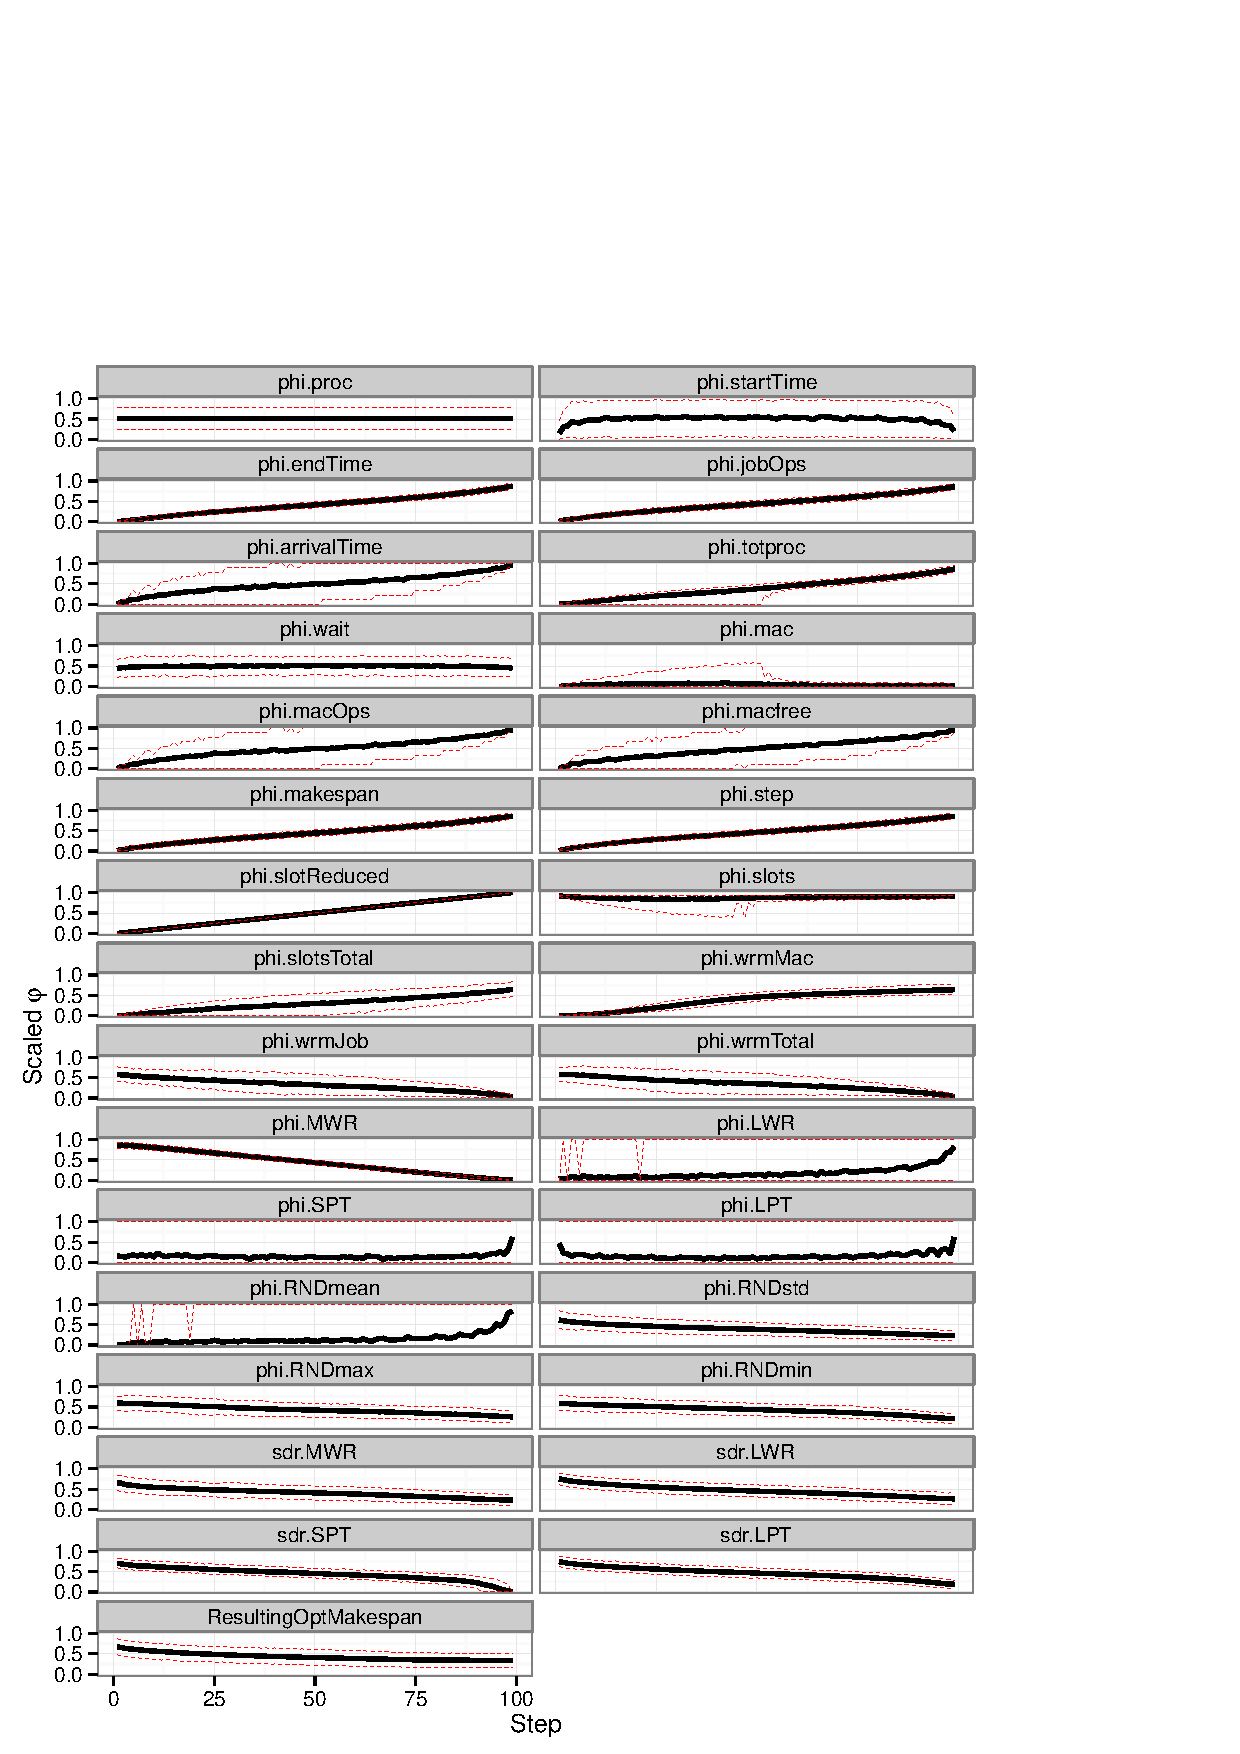
\includegraphics[height=0.9\textheight]{{figures/j.rnd/trdat.feat.stepwise.10x10.OPT}.pdf}}
\end{figure}
\begin{figure}\ContinuedFloat
	\centering
	\subfloat[SPT trajectory]{
		\includegraphics[height=0.9\textheight]{{figures/j.rnd/trdat.feat.stepwise.6x5.SPT}.pdf}}
\end{figure}
\begin{figure}\ContinuedFloat
	\centering
	\subfloat[LPT trajectory]{
		\includegraphics[height=0.9\textheight]{{figures/j.rnd/trdat.feat.stepwise.6x5.LPT}.pdf}}
\end{figure}
\begin{figure}\ContinuedFloat
	\centering
	\subfloat[MWR trajectory]{
		\includegraphics[height=0.9\textheight]{{figures/j.rnd/trdat.feat.stepwise.6x5.MWR}.pdf}}
\end{figure}
\begin{figure}\ContinuedFloat
	\centering
	\subfloat[LWR trajectory]{
		\includegraphics[height=0.9\textheight]{{figures/j.rnd/trdat.feat.stepwise.6x5.LWR}.pdf}}
\end{figure}

\subsection{Variance within distribution}
\begin{figure}
	\subfloat[SPT trajectory]{
		\begin{minipage}{\textwidth}
			\includegraphics[width=\textwidth]{{figures/j.rnd/trdat.feat.KSmatrix.stepwise.EasyVsHard.6x5.SPT}.pdf}
			\\
			\includegraphics[width=\textwidth]{{figures/j.rnd/trdat.feat.corrmatrix.stepwise.EasyVsHard.6x5.SPT}.pdf}
		\end{minipage}}
	\caption{P-values whether features for easy and hard problems are drawn from the same data distribution (above) and significant correlation for features and resulting \namerho, (below) over various trajectories.
		}\label{tbl:easyhard:jrnd} 
\end{figure}
\begin{figure}\ContinuedFloat 
	\subfloat[LPT trajectory]{
		\begin{minipage}{\textwidth}
			\includegraphics[width=\textwidth]{{figures/j.rnd/trdat.feat.KSmatrix.stepwise.EasyVsHard.6x5.LPT}.pdf}\\
			\includegraphics[width=\textwidth]{{figures/j.rnd/trdat.feat.corrmatrix.stepwise.EasyVsHard.6x5.LPT}.pdf}
		\end{minipage}}
\end{figure}
\begin{figure}\ContinuedFloat
	\subfloat[MWR trajectory]{
		\begin{minipage}{\textwidth}
			\includegraphics[width=\textwidth]{{figures/j.rnd/trdat.feat.KSmatrix.stepwise.EasyVsHard.6x5.MWR}.pdf}}
		\\
		\includegraphics[width=\textwidth]{{figures/j.rnd/trdat.feat.corrmatrix.stepwise.EasyVsHard.6x5.MWR}.pdf}
	\end{minipage}}
\end{figure}
\begin{figure}\ContinuedFloat 
	\subfloat[LWR trajectory]{
		\begin{minipage}{\textwidth}
			\includegraphics[width=\textwidth]{{figures/j.rnd/trdat.feat.corrmatrix.stepwise.EasyVsHard.6x5.LWR}.pdf}
			\\
			\includegraphics[width=\textwidth]{{figures/j.rnd/trdat.feat.KSmatrix.stepwise.EasyVsHard.6x5.LWR}.pdf}
		\end{minipage}}
\end{figure}


\subsection{Probability of optimality}
\begin{figure}
	\subfloat[Probability a dispatch is optimal, stepwise (solid) and sequential\footnote{Assuming independant probablity for each stepwise dispatch.} (dashed).]{
		\includegraphics[width=\textwidth]{{figures/j.rnd/trdat.prob.moveIsOptimal.6x5.OPT}.pdf}
	}
	\\
	\subfloat[Probability of optimal dispatch being equivalent to SDRs]{
		\includegraphics[width=\textwidth]{{figures/j.rnd/trdat.prob.moveIsOptimal.SDR.6x5}.pdf}
	}
	\caption{Probability of dispatches begin optimal (above) and optimal dispatches begin equivalent to SDRs (below).}
\end{figure}

\subsection{Ranking}
\begin{figure}
	\subfloat[Ranking of dispathces]{
		\includegraphics[width=\textwidth]{{figures/j.rnd/trdat.rank.6x5.OPT}.pdf}
	}
	\\
	\subfloat[Ranking of dispatches chosen by SDRs]{
		\includegraphics[width=\textwidth]{{figures/j.rnd/trdat.rankSDR.6x5}.pdf}
	}
	\caption{Ranking as function of dispatch iteration, where lower ranking is preferred as rank 0 corresponds to optimal decision.}
\end{figure}

\clearpage
\section{JSP random-narrow}\label{sec:easyhard:jrndn}
\subsection{Evolution of features}
\begin{figure}
	\centering
	\subfloat[Optimum trajectory]{
		\includegraphics[height=0.9\textheight]{{figures/j.rndn/trdat.feat.stepwise.6x5.OPT}.pdf}}
	\caption{Stepwise evolution of (scaled) features w.r.t. various trajectories.}
\end{figure}
\begin{figure}\ContinuedFloat
	\centering
	\subfloat[SPT trajectory]{
		\includegraphics[height=0.9\textheight]{{figures/j.rndn/trdat.feat.stepwise.6x5.SPT}.pdf}}
\end{figure}
\begin{figure}\ContinuedFloat
	\centering
	\subfloat[LPT trajectory]{
		\includegraphics[height=0.9\textheight]{{figures/j.rndn/trdat.feat.stepwise.6x5.LPT}.pdf}}
\end{figure}
\begin{figure}\ContinuedFloat
	\centering
	\subfloat[MWR trajectory]{
		\includegraphics[height=0.9\textheight]{{figures/j.rndn/trdat.feat.stepwise.6x5.MWR}.pdf}}
\end{figure}
\begin{figure}\ContinuedFloat
	\centering
	\subfloat[LWR trajectory]{
		\includegraphics[height=0.9\textheight]{{figures/j.rndn/trdat.feat.stepwise.6x5.LWR}.pdf}}
\end{figure}

\subsection{Variance within distribution}
\begin{figure}
	\subfloat[SPT trajectory]{
		\begin{minipage}{\textwidth}
			\includegraphics[width=\textwidth]{{figures/j.rndn/trdat.feat.KSmatrix.stepwise.EasyVsHard.6x5.SPT}.pdf}
			\\
			\includegraphics[width=\textwidth]{{figures/j.rndn/trdat.feat.corrmatrix.stepwise.EasyVsHard.6x5.SPT}.pdf}
		\end{minipage}}
	\caption{P-values whether features for easy and hard problems are drawn from the same data distribution (above) and significant correlation for features and resulting \namerho, (below) over various trajectories.
		}\label{tbl:easyhard:jrndn} 
\end{figure}
\begin{figure}\ContinuedFloat 
	\subfloat[LPT trajectory]{
		\begin{minipage}{\textwidth}
			\includegraphics[width=\textwidth]{{figures/j.rndn/trdat.feat.KSmatrix.stepwise.EasyVsHard.6x5.LPT}.pdf}\\
			\includegraphics[width=\textwidth]{{figures/j.rndn/trdat.feat.corrmatrix.stepwise.EasyVsHard.6x5.LPT}.pdf}
		\end{minipage}}
\end{figure}
\begin{figure}\ContinuedFloat
	\subfloat[MWR trajectory]{
		\begin{minipage}{\textwidth}
			\includegraphics[width=\textwidth]{{figures/j.rndn/trdat.feat.KSmatrix.stepwise.EasyVsHard.6x5.MWR}.pdf}}
		\\
		\includegraphics[width=\textwidth]{{figures/j.rndn/trdat.feat.corrmatrix.stepwise.EasyVsHard.6x5.MWR}.pdf}
	\end{minipage}}
\end{figure}
\begin{figure}\ContinuedFloat 
	\subfloat[LWR trajectory]{
		\begin{minipage}{\textwidth}
			\includegraphics[width=\textwidth]{{figures/j.rndn/trdat.feat.corrmatrix.stepwise.EasyVsHard.6x5.LWR}.pdf}
			\\
			\includegraphics[width=\textwidth]{{figures/j.rndn/trdat.feat.KSmatrix.stepwise.EasyVsHard.6x5.LWR}.pdf}
		\end{minipage}}
\end{figure}


\subsection{Probability of optimality}
\begin{figure}
	\subfloat[Probability a dispatch is optimal, stepwise (solid) and sequential (dashed).]{
		\includegraphics[width=\textwidth]{{figures/j.rndn/trdat.prob.moveIsOptimal.6x5.OPT}.pdf}
	}
	\\
	\subfloat[Probability of optimal dispatch being equivalent to SDRs]{
		\includegraphics[width=\textwidth]{{figures/j.rndn/trdat.prob.moveIsOptimal.SDR.6x5}.pdf}
	}
	\caption{Probability of dispatches begin optimal (above) and optimal dispatches begin equivalent to SDRs (below).}
\end{figure}

\subsection{Ranking}
\begin{figure}
	\subfloat[Ranking of dispathces]{
		\includegraphics[width=\textwidth]{{figures/j.rndn/trdat.rank.6x5.OPT}.pdf}
	}
	\\
	\subfloat[Ranking of dispatches chosen by SDRs]{
		\includegraphics[width=\textwidth]{{figures/j.rndn/trdat.rankSDR.6x5}.pdf}
	}
	\caption{Ranking as function of dispatch iteration, where lower ranking is preferred as rank 0 corresponds to optimal decision.}
\end{figure}
\end{comment}
